\label{chap:raspberryPi}

La part de la barrera del pàrquing està composta per una Raspberry Pi 4 model B,
una càmera HQ, un LED RGB que simbolitzen les accions de la barrera, tres resistències de 470 Ohms
per fer les connexions amb el LED i per últim un brunzidor elèctric.


\subsection{Connexions}
Aquests components han d'estar connectats a la Raspberry Pi,
seguidament es mostra en els pins que s'han connectat cada un dels LEDs
i el brunzidor. Adjuntant un esquema dels pins de la Raspberry Pi per veure
quins són:

\begin{itemize}
    \item LED Red: GPIO 18
    \item LED Blue: GPIO 23
    \item LED Green: GPIO 24
    \item Brunzidor: GPIO 25
\end{itemize}

\begin{figure}[H]
    \begin{center}
        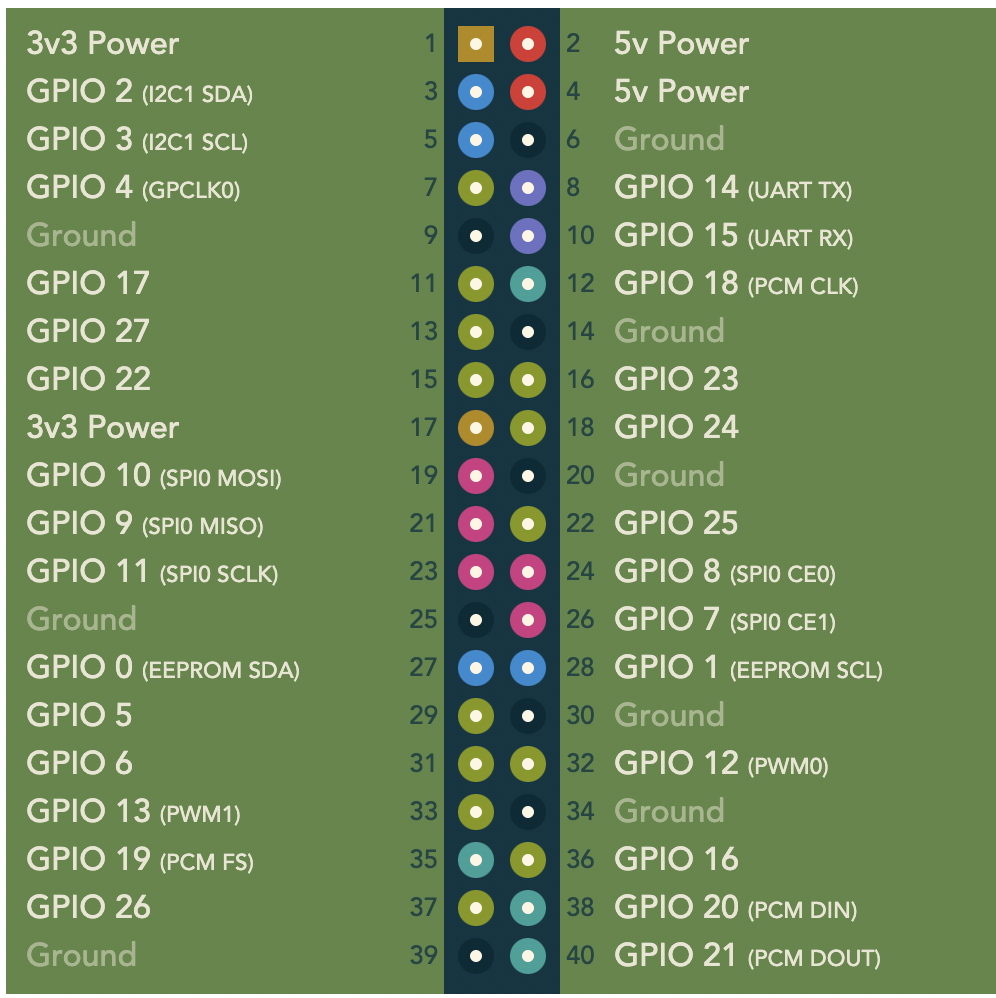
\includegraphics[scale=0.35]{Fotos/rasp_pinout.png}
    \end{center}
    \caption{Raspberry PI 4 pinout}
    \label{fig:payment_photo}
\end{figure}

Finalment, tots els components utilitzats amb el seu muntatge són els següents:

\begin{figure}[H]
    \begin{center}
        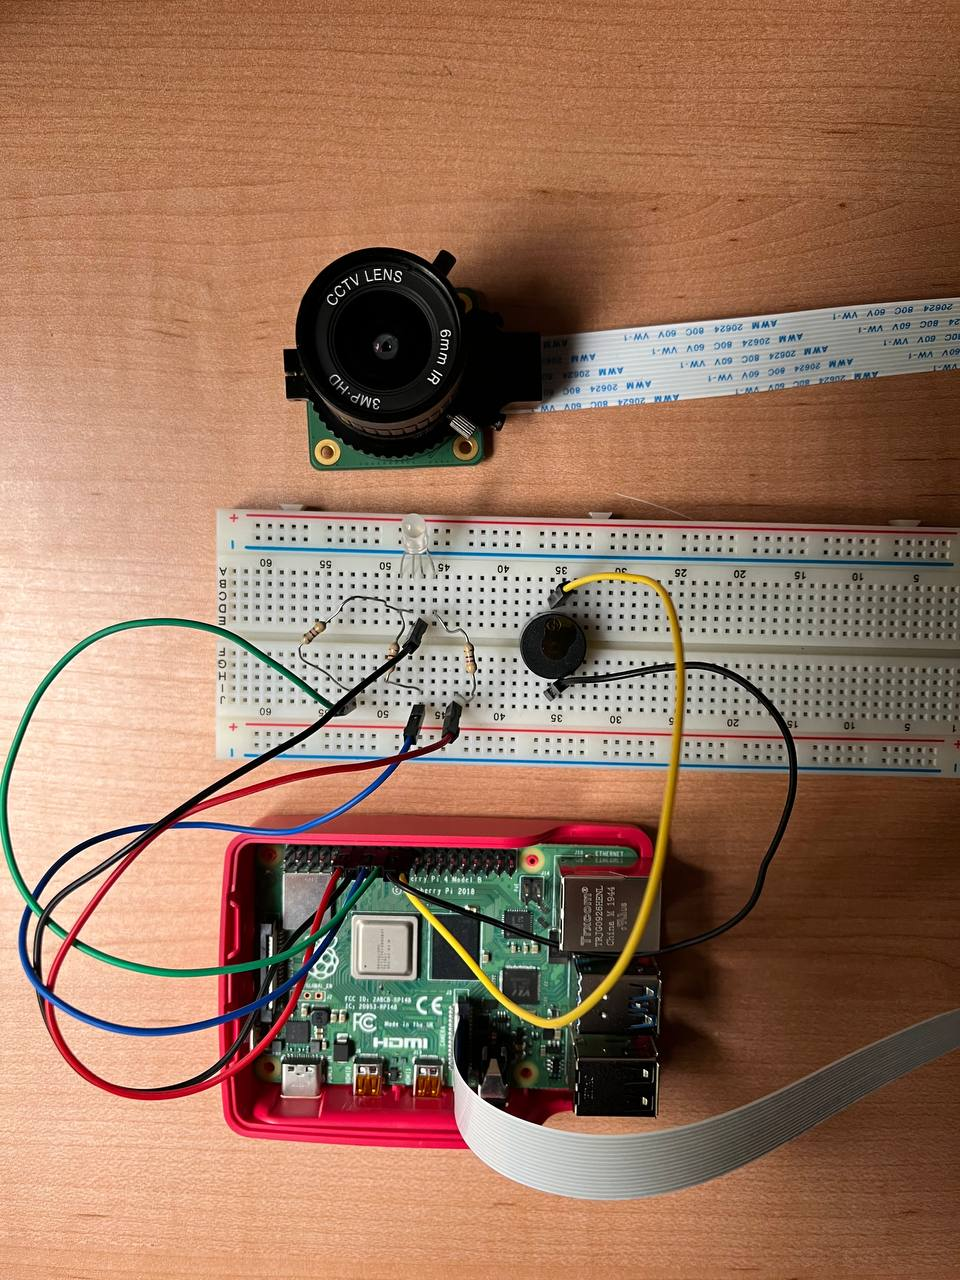
\includegraphics[scale=0.28]{Fotos/material.jpeg}
    \end{center}
    \caption{Muntatge Raspberry Pi}
    \label{fig:material}
\end{figure}


\subsection{Màquina d'estats}

\begin{figure}[H]
\begin{center}
    \includegraphics[scale=0.15]{Fotos/barrera.png}
\end{center}
\caption{Màquina d'estat detecció codi QR}
\label{fig:maq_estats}
\end{figure}

\begin{enumerate}
    \item \texttt{Estat 0}: Indica que la barrera està baixada posant el LED de color vermell a \emph{ON}.
    Obra la càmera connectada a la Raspberry Pi on es prepara per detectar codis QR.
    Quan en detecta un llegeix el seu contingut i el guarda a la variable anomenada
    \emph{qr}.
    Deshabilita la càmera, d'aquesta manera no pot detectar més codis QR.
    Quan detecta el codi QR s'activa el brunzidor que dura cinc segons i canvia al següent estat, l'estat 1.
    \item \texttt{Estat 1}: Es deshabilita el brunzidor. Apaga el LED vermell i posa a \emph{ON} el LED blau, ja
    que aquest LED indica que està fent la petició HTTP. Es guarda la resposta d'aquesta petició
    a una variable anomenada \emph{respostaHTTP}. Canvia al següent estat, l'estat 2.
    \item \texttt{Estat 2}: Apaga el LED blau, i comprova la resposta HTTP. Si la resposta
    és \texttt{204}, canvia l'estat a Estat 4. Si no ho és, canvia l'estat a l'estat 3.
    \item \texttt{Estat 3}: Per indicar a l'usuari que la resposta no ha sigut
    satisfactòria, el LED vermell farà quatre pampallugues.
    Finalment, l'estat passa a ser l'estat inicial, l'estat 0.
    \item \texttt{Estat 4}: Aquest estat és quan la resposta HTTP ha sigut satisfactòria.
    En aquest estat el LED Verd farà quatre pampallugues indicant que la barrera està pujant.
    Quan la barrera ha pujat, l'estat passa a ser l'estat 5.
    \item \texttt{Estat 5}: Posa el LED verd a \emph{ON}. Simbolitza la barrera pujada.
    Quan ha passat el temps corresponent canvia l'estat a l'estat 6.
    \item \texttt{Estat 6}: Aquest estat es comporta igual que l'estat 4. El LED Verd
    fa quatre pampallugues per indicar que la barrera està baixant.
    Quan es troba a abaixada passa a l'estat inicial. L'estat 0.
\end{enumerate}


\subsubsection{Llibreries}
Les llibreries utilitzades per fer la màquina d'estats anteriors
són les següents:
\begin{itemize}
    \item Requests: per fer peticions HTTP \autocite{requests}.
    \item Enum: Per declarar els estats \autocite{enum_python}. Tot i que aquesta llibreria
    és de la llibreria estàndard de Python.
    \item Time: Per fer la durada. S'utilitza la funció \emph{sleep()}. Tot i que aquesta llibreria
    és de la llibreria estàndard de Python.
    Com que el codi no fa res més no passa res que sigui bloquejant \autocite{sleep_python}
    \item RPi.GPIO: Per configurar els inputs de la Raspberry Pi \autocite{gpio_rasp}.
    \item cv2: Per obrir la càmera \autocite{cv2}.
    \item Pyzbar: Detectar codis QR, llegir-los i descodificar-los \autocite{pyzbar}.
\end{itemize}

